\documentclass[../main.tex]{subfiles}

\begin{document}

To finalize our insight into how PNC works, we need to describe the build process from a high-level perspective:
\begin{enumerate}
    \item \textbf{Trigger a build}\\
    A build is triggered (almost exclusively) either from PNC UI or Bacon CLI. In both cases, this results in Orch's trigger build endpoint being called. Every build is configured by its build configuration containing all the necessary information, e.g.:
    \begin{itemize}
        \item \textbf{repository:} repository with source code, e.g. \url{https://github.com/wildfly/wildfly}
        \item \textbf{git reference:} (branch, tag or commit) revision which will be used to clone source code, e.g. \textit{34.0.0.Final}
        \item \textbf{build type:} either Maven, Gradle, NPM, or SBT
        \item \textbf{build environment:} the build environment used in build container
        \item \textbf{build script:} a script executed in the build container, e.g. \textit{mvn clean deploy}
    \end{itemize}

    \item \textbf{Start an alignment}\\
    Repour clones specified repository locally into the container environment in which it runs. Subsequently, it starts the alignment operation by calling the corresponding manipulator based on the build type (for instance, for the Maven build type, the PME manipulator is picked).

    \item \textbf{Alignment process}\\
    A manipulator configured from Repour communicates with DA to perform both version increment and dependencies alignment.

    \item \textbf{Push alignment changes}\\
    Once the manipulator successfully finishes, alignment changes are pushed into a downstream repository.

    \item \textbf{Create a build container}\\
    Create the environment for the build itself based on the build environment from the build configuration.

    \item \textbf{Clone alignment changes}\\
    Before a build container runs the build itself, it needs to clone alignment changes from the downstream repository pushed by Repour in step 4.

    \item \textbf{Run a build}\\
    Run the build script from a build configuration. During a build, a build container communicates with an artifact repository in order to fetch artifacts.

    \item \textbf{Store built artifacts}\\
    Once a build succeeds, its produced artifacts need to be stored in the artifact repository in order to be accessible by subsequent builds.

    \item \textbf{Save the build result into DB}\\
    Save all the build-related data into the orch database. This holds information like used build configuration, artifacts produced by the build, or artifacts used by the build.
    
\end{enumerate}

The whole build process is also visualized by BPMN diagram\footnote{\url{https://miro.com/diagramming/what-is-bpmn/}} shown in the Figure \ref{fig:build-process-bpmn}.\\
\textbf{Note:} Even though the BPM microservice manages the whole process, it is shown neither in the text description nor in Figure \ref{fig:build-process-bpmn} in order to prevent showing all the unnecessary details.

\begin{figure}
  \begin{center}
    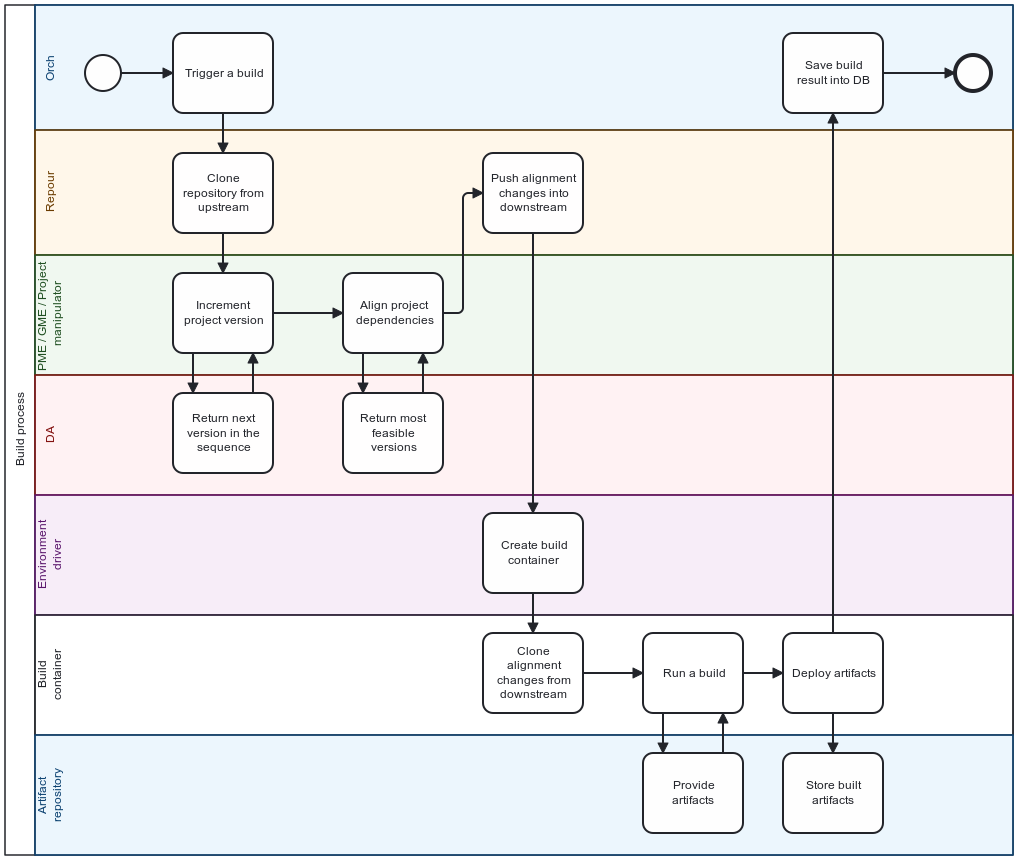
\includegraphics[width=\textwidth]{images/build-process-bpmn.png}
  \end{center}
  \caption{BPMN build process diagram}
  \label{fig:build-process-bpmn}
\end{figure}

\end{document}
